\documentclass{beamer}
\usepackage{cmap} % поиск и копирование в PDF документах
\usepackage[T2A]{fontenc}
\usepackage[english,russian]{babel}
\usepackage[utf8]{inputenc}
% Стиль презентации
\usetheme{Warsaw}

\hypersetup{
  colorlinks=true,
  linkcolor=white,    
  urlcolor=cyan,
}

\begin{document}
  % Слайд: название статьи
  \title{Обнаружение текста при помощи Глубоких Нейронных Сетей}  
  \author{Деин Евгений}
  \institute{ИРИТ-РТФ}
  \date{Екатеринбург, 2017} 
  
  % Создание заглавной страницы
  \frame{\titlepage} 
  
  % Слайд: цели
  \begin{frame}{Цели статьи}
    \begin{itemize}
      \item{Познакомить читателя с архитектурой ICPT-CNN}
      \item{Познакомить читателя с обучением ICPT-CNN}
      \item{Сравнить с другими алгоритмами рассматриваемую архитектуру}
    \end{itemize}
  \end{frame}

  % Слайд: архитектура CNN
  \begin{frame}{Архитектура CNN}
    \begin{center}
      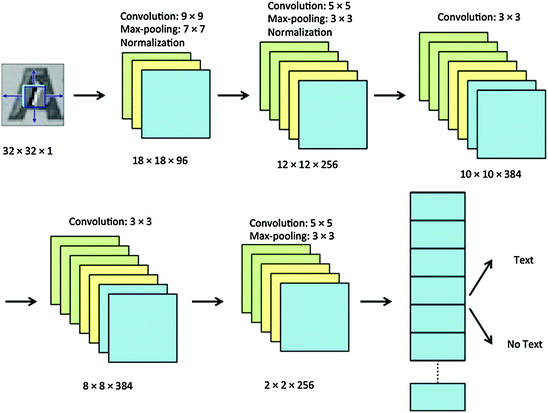
\includegraphics[scale=0.3]{cnn-architec.jpg}
    \end{center}
    \begin{block}{ICPT-CNN}
      CNN с улучшенной технологией последующей свертки
    \end{block}
    \begin{block}{Вход --> Выход}
      Картинка --> Есть текст/Нет текста
    \end{block}
  \end{frame}

  % Слайд: пример обучающей выборки
  \begin{frame}{Пример обучающей выборки}
    Размер картинок из датасета     \href{http://www.iapr-tc11.org/mediawiki/index.php/ICDAR_2003_Robust_Reading_Competitions}{ICDAR 2003-2005} -- 32x32
    \begin{center}
      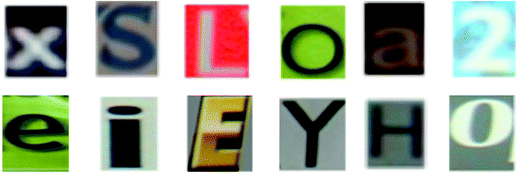
\includegraphics[scale=0.5]{samples.jpg}
    \end{center}
  \end{frame}

  % Слайд: блок-схема
  \begin{frame}{Блок-схема}
    \begin{center}
      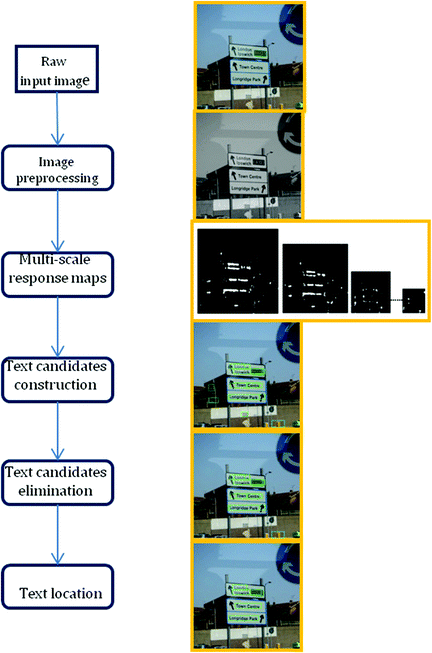
\includegraphics[scale=0.35]{flowchart.jpg}
    \end{center}
  \end{frame}

  % Слайд: заключение
  \begin{frame}{Заключение}
    \begin{itemize}
      \item{Алгоритм ICPT-CNN был успешно реализован}
      \pause
      \item{Алгоритм был улучшен(ReLU, скрытые признаки)}
      \pause
      \item{Результаты ICPT-CNN были лучшими из всех алгоритмов}
    \end{itemize}
  \end{frame}
\end{document}